\newpage
\section{File System Implementation}

\subsection{File-System Structure}
File structure: 需要解决接口与内部数据结构. 
\begin{itemize}
    \item Logical storage unit
    \item Collection of related information
\end{itemize}
File system resides on secondary storage (disks). File system organized into layers. 

\begin{figure}[!htb]
    \centering
    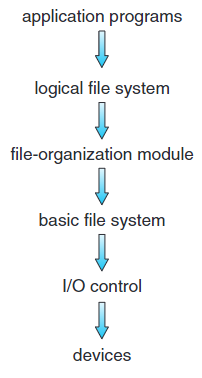
\includegraphics[width=0.22\textwidth]{pic/OS11/Layered file system}
    \caption{Layered file system}
\end{figure}

\begin{table}[!htb]
    \centering
    \caption{Layered file system}\tiny
    \begin{tabular}[c]{cc}\toprule
         \\ \midrule 
        logical file system& \begin{tabular}[c]{@{}l@{}}Manages metadata of files. \\ Protection and security\end{tabular} \\
        file-organization module& \begin{tabular}[c]{@{}l@{}}Translates logical block addr to physical addr. \\ Free space mgmt\end{tabular}\\
        basic file system & Commands to r/w physical blocks\\
        I/O control & Translates `r/w block' to low-level hw instructions\\
        \bottomrule
    \end{tabular}
\end{table}

FTL (flash) is I/O control

\subsection{File-System Implementation}
\subsubsection{Data Structures Used to Implement FS}
Disk structures:
\begin{itemize}
    \item Boot control block
    \item Volume control block (superblock in Unix)
    \item Directory structure per file system
    \item Per-file FCB (inode in Unix)
\end{itemize}
In-memory structures:
\begin{itemize}
    \item In-memory mount table about each mounted volume
    \item Directory cache
    \item System-wide open-file table
    \item Per-process open-file table
\end{itemize}

\begin{figure}[!htb]
    \centering
    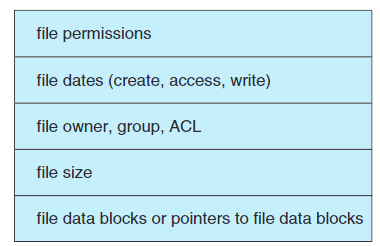
\includegraphics[width=0.22\textwidth]{pic/OS11/A typical file-control block}
    \caption{A typical file-control block: storage structure consisting of information about a file}
\end{figure}

\begin{figure}[!htb]
    \centering
    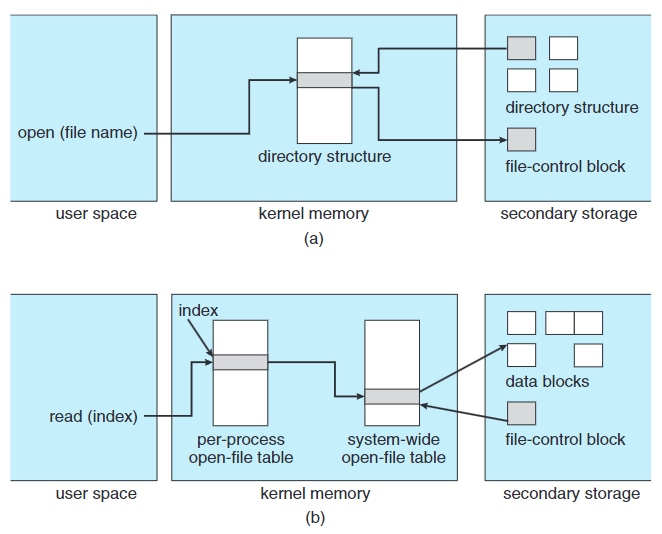
\includegraphics[width=0.42\textwidth]{pic/OS11/In-memory file-system structures.}
    \caption{In-memory file-system structures.(a) File open. (b) File read.}
\end{figure}

\subsubsection{Virtual File Systems}
Virtual File Systems (VFS) provide an object-oriented way of implementing file systems. VFS isn't a disk file system. 

VFS allows the same system call interface (the API) to be used for different types of file systems.

Defines a network-wide unique structure called vnode. 

VFS is logical file system

\begin{figure}[!htb]%TODO 去边框 11.11
    \centering
    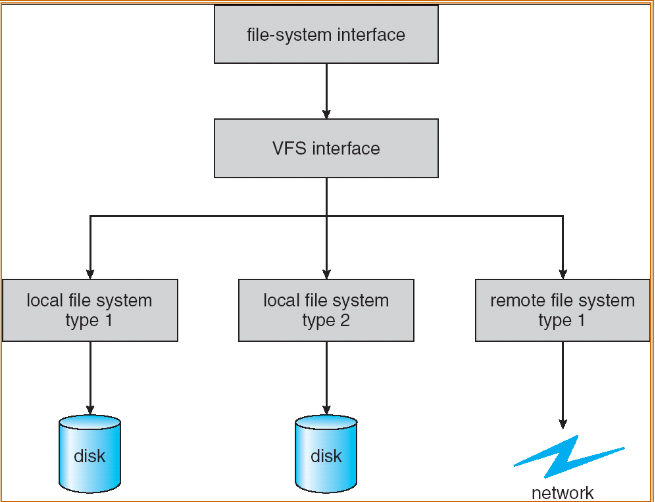
\includegraphics[width=0.309\textwidth]{pic/OS11/Schematic View of Virtual File System}
    \caption{Schematic View of Virtual File System}
\end{figure}

\subsection{Directory Implementation}
Linear list of file names with pointer to the data blocks
\begin{itemize}
    \item simple to program
    \item time-consuming to execute
\end{itemize}

Hash Table: linear list with hash data structure
\begin{itemize}
    \item decreases directory search time
    \item collisions: situations where two file names hash to the same
    location
    \item fixed size: can use chained-overflow hash table
\end{itemize}

\subsection{Allocation Methods}
An allocation method refers to how disk blocks are allocated for files. 

\subsubsection{Contiguous allocation}
Each file occupies a set of contiguous blocks on the disk. But it's Wasteful of space (dynamic storage-allocation problem). Random access supported

Mapping from logical to physical: 
\begin{align*}
    \text{Logic Address}=512Q+R
\end{align*}
\begin{itemize}
    \item Block to be accessed $=Q+$ start address
    \item Displacement into block $=R$
\end{itemize}

\paragraph*{Extent-Based Systems} a modified contiguous allocation scheme. 

Extent-based file systems allocate disk blocks in extents.  An extent is a contiguous block of disks. 

\subsubsection{Linked allocation}
Each file is a linked list of disk blocks: blocks may be scattered anywhere on the disk. No random access, poor reliability

\begin{figure}[!htb]
    \centering
    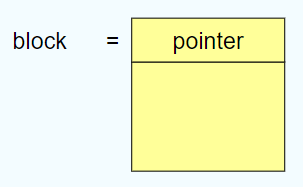
\includegraphics[width=0.22\textwidth]{pic/OS11/Linked Allocation}
    \caption{Linked Allocation}
\end{figure}

Mapping: 
\begin{align*}
    \text{Logic Address}=511Q+(R-1)
\end{align*}
511 because of pointer
\begin{itemize}
    \item Block to be accessed is the Qth block in the linked chain of
    blocks representing the file
    \item Displacement into block $=R+1$
\end{itemize}

\begin{figure}[!htb]
    \centering
    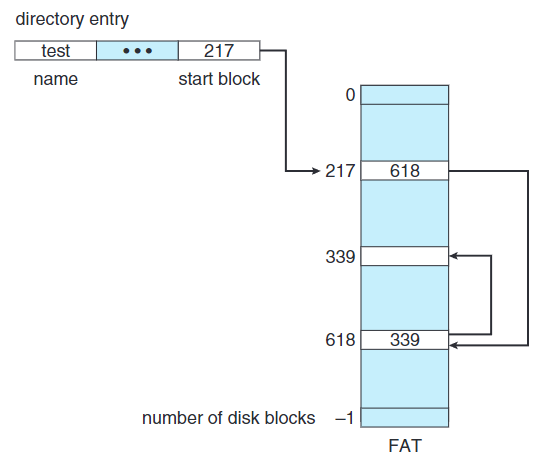
\includegraphics[width=0.309\textwidth]{pic/OS11/File-allocation table}
    \caption{File-allocation table(改进的 Linked Allocation, 将 linked 放入内存)}
\end{figure}

\subsubsection{Indexed allocation}
Brings all pointers together into the index block. Random access
\begin{figure}[!htb]
    \centering
    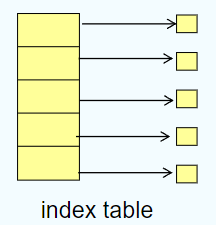
\includegraphics[width=0.22\textwidth]{pic/OS11/Indexed allocation}
    \caption{Indexed allocation}
\end{figure}

Mapping: 
\begin{enumerate}
    \item When mapping from logical to physical in a file of maximum
    size of 256K words and block size of 512 words. We need
    only 1 block for index table
    \begin{align*}
        \text{Logic Address}=512Q+R
    \end{align*}
    \begin{itemize}
        \item $Q =$ displacement into index table
        \item $R =$ displacement into block
    \end{itemize}
    \item When mapping from logical to physical in a file of
    unbounded length (block size of 512 words). -- more
    pointers are needed
    \begin{align*}
        \text{Logic Address}&=(512\times 511)Q_1+R_1\\
        R_1&=512Q_2+R_2
    \end{align*}
    \begin{itemize}
        \item Linked scheme - Link blocks of index table
        \subitem $Q_1=$ block of index table
        \subitem $Q_2=$ displacement into block of index table
        \subitem $R_2=$ displacement into block of file
        \item Two-level index
        \subitem $Q_1=$ displacement into outer-index
        \subitem $Q_2=$ displacement into block of index table
        \subitem $R_2=$ displacement into block of file
    \end{itemize}
\end{enumerate}

\begin{figure}[!htb]
    \centering
    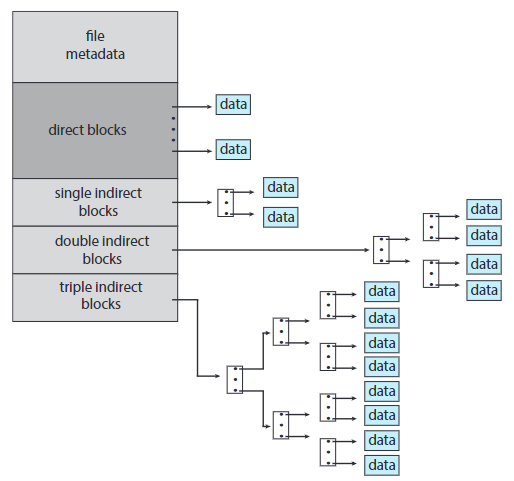
\includegraphics[width=0.42\textwidth]{pic/OS11/The UNIX inode}
    \caption{The UNIX inode(Combined Scheme)}
\end{figure}


\subsection{Free-Space Management}
\begin{figure}[!htb]
    \centering
    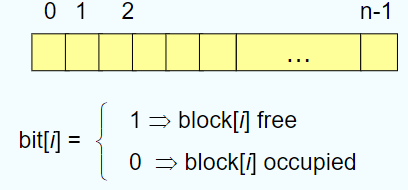
\includegraphics[width=0.309\textwidth]{pic/Os11/Bit vector}
    \caption{Bit vector}
\end{figure}

e.g. %TODO P30

\begin{itemize}
    \item Linked list (free list) 
    \item Grouping: a modification of the Linked List
    \item Counting: Address of the first free block and number n contiguous blocks
\end{itemize}

\subsection{Efficiency and Performance}
Efficiency dependent on:
\begin{itemize}
    \item disk allocation and directory algorithms
    \item types of data kept in file's directory entry
\end{itemize}
Generally, every data item has to be considered for its effect. 


Performance:
\begin{itemize}
    \item disk cache: separate section of main memory for frequently
    used blocks
    \item free-behind and read-ahead: techniques to optimize
    sequential access
    \item improve PC performance by dedicating section of memory as
    virtual disk, or RAM disk
\end{itemize}


\subsubsection{Page Cache}
A page cache caches pages rather than disk blocks using virtual
memory techniques. 

将 page cache 与 buffer cache 合并. 